\documentclass[11pt,a4paper,oneside]{report}
\usepackage{amsmath,amssymb,calc,ifthen}
\usepackage{float}
%\usepackage{cancel}
\usepackage[table,usenames,dvipsnames]{xcolor} % for coloured cells in tables
\usepackage{tikz}
% Allows us to click on links and references!
\usepackage{hyperref}
\usepackage{url}
\hypersetup{
colorlinks,
citecolor=black,
filecolor=black,
linkcolor=black,
urlcolor=black
}
% Nice package for plotting graphs
% See excellent guide:
% http://www.tug.org/TUGboat/tb31-1/tb97wright-pgfplots.pdf
\usetikzlibrary{plotmarks}
\usepackage{amsmath,graphicx}
\usepackage{epstopdf}
\usepackage{caption}
\usepackage{bbm}
\usepackage{subcaption}
% highlight - useful for TODOs and similar
\usepackage{color}
\newcommand{\hilight}[1]{\colorbox{yellow}{#1}}
\newcommand\ci{\perp\!\!\!\perp} % perpendicular sign
\newcommand*\rfrac[2]{{}^{#1}\!/_{#2}} % diagonal fraction
\newcommand\SLASH{\char`\\}
\usepackage{listings}
% margin size
\usepackage[margin=1in]{geometry}
\tikzstyle{state}=[circle,thick,draw=black, align=center, minimum size=2.1cm,
inner sep=0]
\tikzstyle{vertex}=[circle,thick,draw=black]
\tikzstyle{terminal}=[rectangle,thick,draw=black]
\tikzstyle{edge} = [draw,thick]
\tikzstyle{lo} = [edge,dotted]
\tikzstyle{hi} = [edge]
\tikzstyle{trans} = [edge,->]
\definecolor{mygreen}{rgb}{0,0.6,0}
\definecolor{mygray}{rgb}{0.5,0.5,0.5}
\definecolor{mymauve}{rgb}{0.58,0,0.82}
\DeclareMathOperator*{\argmin}{arg\,min}
\DeclareMathOperator*{\argmax}{arg\,max}
\newcommand*{\Comb}[2]{{}^{#1}C_{#2}}
\lstset{ %
backgroundcolor=\color{white}, % choose the background color; you must add
%\usepackage{color} or \usepackage{xcolor}
basicstyle=\footnotesize, % the size of the fonts that are used for the
%code
breakatwhitespace=false, % sets if automatic breaks should only happen
%at whitespace
breaklines=true, % sets automatic line breaking
captionpos=b, % sets the caption-position to bottom
commentstyle=\color{mygreen}, % comment style
deletekeywords={...}, % if you want to delete keywords from the
%given language
escapeinside={\%*}{*)}, % if you want to add LaTeX within your code
extendedchars=true, % lets you use non-ASCII characters; for
%8-bits encodings only, does not work with UTF-8
frame=single, % adds a frame around the code
keepspaces=true, % keeps spaces in text, useful for keeping
%indentation of code (possibly needs columns=flexible)
keywordstyle=\color{blue}, % keyword style
language=Octave, % the language of the code
morekeywords={*,...}, % if you want to add more keywords to the set
numbers=left, % where to put the line-numbers; possible
%values are (none, left, right)
numbersep=5pt, % how far the line-numbers are from the code
numberstyle=\tiny\color{mygray}, % the style that is used for the line-numbers
rulecolor=\color{black}, % if not set, the frame-color may be changed
%on line-breaks within not-black text (e.g. comments (green here))
showspaces=false, % show spaces everywhere adding particular
%underscores; it overrides 'showstringspaces'
showstringspaces=false, % underline spaces within strings only
showtabs=false, % show tabs within strings adding particular
%underscores
stepnumber=2, % the step between two line-numbers. If it's
%1, each line will be numbered
stringstyle=\color{mymauve}, % string literal style
tabsize=2, % sets default tabsize to 2 spaces
title=\lstname % show the filename of files included with
%\lstinputlisting; also try caption instead of title
}
\title{Graphical Models Coursework 3}
\author{
Razvan Valentin Marinescu\\
Student Number: 14060166\\
\texttt{razvan.marinescu.14@ucl.ac.uk}
\and
Konstantinos Georgiadis\\
Student Number: 14110861\\
\texttt{konstantinos.georgiadis.14@ucl.ac.uk}
}
\begin{document}
\belowdisplayskip=12pt plus 3pt minus 9pt
\belowdisplayshortskip=7pt plus 3pt minus 4pt
\maketitle{}

Just as in the previous assignment, we both did the exercises independently and compared our answers until we agreed on what to choose. Konstantinos wrote most of the report and Razvan added some changes afterwards.

\section*{Exercise 7.4}

We changed the code from demoMDP accordingly for this exercise and we only kept the Value Iteration strategy. We kept the value of gamma to be the same as it was (0.95), as well as the number of iterations to be 30. Our code then proceeds to make moves by moving at each timestep to the neighboring grid position with the highest value and stops once it reaches a point where the grid position that the airplane currently occupies has a higher value than its neighboring grid positions. For the second part of the exercise, we merely had to change the p matrix accordingly. The optimal paths are given from the variable PositionSequence. In the first case, the optimal path is:\\\\
X Y\\
1     13\\
     1    12\\
     1    11\\
     2    11\\
     3    11\\
     4    11\\
     5    11\\
     6    11\\
     7    11\\
     8    11\\
     9    11\\
    10    11\\
    11    11\\
    12    11\\
    13    11\\
    14    11\\
    15    11\\
    15    10\\
    15     9\\
    14     9\\
    14     8\\
    14     7\\
    13     7\\
    12     7\\
    11     7\\
    10     7\\
     9     7\\
     8     7\\
     7     7\\
     6     7\\
     5     7\\
     4     7\\
     4     6\\
     4     5\\
     4     4\\
     5     4\\
     6     4\\
     7     4\\
     8     4\\\\
     
In the second case, the optimal path is:\\\\
X Y\\     
     1    13\\
     1    14\\
     2    14\\
     3    14\\
     4    14\\
     5    14\\
     6    14\\
     7    14\\
     8    14\\
     9    14\\
    10    14\\
    11    14\\
    12    14\\
    13    14\\
    14    14\\
    15    14\\
    16    14\\
    16    13\\
    16    12\\
    16    11\\
    15    11\\
    15    10\\
    15     9\\
    14     9\\
    14     8\\
    14     7\\
    13     7\\
    12     7\\
    11     7\\
    10     7\\
     9     7\\
     8     7\\
     7     7\\
     6     7\\
     5     7\\
     4     7\\
     4     6\\
     4     5\\
     4     4\\
     5     4\\
     6     4\\
     7     4\\
     8     4\\\\
     
     This result can be explained in the sense that the value iteration method makes use of the p matrix, as well as the utility values. Since there is now a higher chance to move up, during the value iterations, the values of the path around the up-right village get higher values, rather than the path through (14,11).\\
     
     MATLAB code:
     

\begin{lstlisting}
clear all;
close all;
load('airplane.mat');
import brml.*
[Gx, Gy] = size(U);  % two dimensional grid size
S = Gx*Gy; % number of states on grid
st = reshape(1:S,Gx,Gy); % assign each grid point a state

A = 5;  % number of action (decision) states
[stay, up, down, left, right] = assign(1:A); % actions (decisions)
p = zeros(S,S,A); % initialise the transition p(xt|xtm,dtm) ie p(x(t)|x(t-1),d(t-1))

% make a deterministic transition matrix on a 2D grid:
for x = 1:Gx
	for y = 1:Gy
		p(st(x,y),st(x,y),stay)=1; % can stay in same state
		if validgridposition(x+1,y,Gx,Gy)
			p(st(x+1,y),st(x,y),right)=1;
		end
		if validgridposition(x-1,y,Gx,Gy)
			p(st(x-1,y),st(x,y),left)=1;
		end
		if validgridposition(x,y+1,Gx,Gy)
			p(st(x,y+1),st(x,y),up)=1;
		end
		if validgridposition(x,y-1,Gx,Gy)
			p(st(x,y-1),st(x,y),down)=1;
		end
	end
end
% define utilities
u = U(:);
gamma = 0.95; % discount factor
figure; imagesc(reshape(u,Gx,Gy)); colorbar; title('utilities');
[xt, xtm, dtm]=assign(1:3); % assign the variables x(t), x(t-1), d(t-1) to some numbers

% define the transition potentials p(x(t)|x(t-1),d(t-1))
tranpot=array([xt xtm dtm],p);
% setup the value potential v(x(t))
valpot=array(xt,ones(S,1)); % initial values

maxiterations=30; tol=0.001; % termination criteria
% Value Iteration:
oldvalue=valpot.table;
for valueloop=1:maxiterations
	valueloop
	tmppot = maxpot(sumpot(multpots([tranpot valpot]),xt),dtm);
	valpot.table = u + gamma*tmppot.table; % Bellman's recursion
	if mean(abs(valpot.table-oldvalue))<tol; break; end % stop if converged
	oldvalue = valpot.table;
	imagesc(reshape(valpot.table,Gx,Gy)); colorbar; drawnow
end
figure; bar3zcolor(reshape(valpot.table,Gx,Gy));

FinalValues = reshape(valpot.table,Gx,Gy);

%Calculate Optimal Sequence
PositionSequence = [1 13];
timestep = 1;
while(1)
    x = PositionSequence(timestep,1);
    y = PositionSequence(timestep,2);
    %find best move
    currentval = FinalValues(x,y);
    bestmove = stay;
    if validgridposition(x+1,y,Gx,Gy)
        if(FinalValues(x+1,y) > currentval)
            currentval = FinalValues(x+1,y);
            bestmove = right;
        end
    end
    if validgridposition(x-1,y,Gx,Gy)
        if(FinalValues(x-1,y) > currentval)
            currentval = FinalValues(x-1,y);
            bestmove = left;
        end
    end
    if validgridposition(x,y+1,Gx,Gy)
        if(FinalValues(x,y+1) > currentval)
            currentval = FinalValues(x,y+1);
            bestmove = up;
        end
    end
    if validgridposition(x,y-1,Gx,Gy)
        if(FinalValues(x,y-1) > currentval)
            currentval = FinalValues(x,y-1);
            bestmove = down;
        end
    end
    %make new move or exit
    timestep = timestep + 1;
    if(bestmove == stay)
        break;
    end
    PositionSequence(timestep,1:2) = PositionSequence(timestep-1,1:2);
    if(bestmove == right)
        PositionSequence(timestep,1) = PositionSequence(timestep,1)+1;
    end
    if(bestmove == left)
        PositionSequence(timestep,1) = PositionSequence(timestep,1)-1;
    end
    if(bestmove == up)
        PositionSequence(timestep,2) = PositionSequence(timestep,2)+1;
    end
    if(bestmove == down)
        PositionSequence(timestep,2) = PositionSequence(timestep,2)-1;
    end
end
PositionSequence



%Part 2
p = zeros(S,S,A); 
for x = 1:Gx
	for y = 1:Gy
		p(st(x,y),st(x,y),stay)=1; 
		if validgridposition(x+1,y,Gx,Gy)
            if validgridposition(x,y+1,Gx,Gy)
                p(st(x+1,y),st(x,y),right)=0.9;
                p(st(x,y+1),st(x,y),right)=0.1;
            else
                p(st(x+1,y),st(x,y),right)=1;
            end
		end
		if validgridposition(x-1,y,Gx,Gy)
			p(st(x-1,y),st(x,y),left)=1;
		end
		if validgridposition(x,y+1,Gx,Gy)
			p(st(x,y+1),st(x,y),up)=1;
		end
		if validgridposition(x,y-1,Gx,Gy)
			p(st(x,y-1),st(x,y),down)=1;
		end
	end
end
% define utilities
u = U(:);
gamma = 0.95;
figure; imagesc(reshape(u,Gx,Gy)); colorbar; title('utilities');
[xt, xtm, dtm]=assign(1:3); % assign the variables x(t), x(t-1), d(t-1) to some numbers

% define the transition potentials p(x(t)|x(t-1),d(t-1))
tranpot=array([xt xtm dtm],p);
% setup the value potential v(x(t))
valpot=array(xt,ones(S,1)); % initial values

maxiterations=30; tol=0.001; % termination criteria
% Value Iteration:
oldvalue=valpot.table;
for valueloop=1:maxiterations
	valueloop
	tmppot = maxpot(sumpot(multpots([tranpot valpot]),xt),dtm);
	valpot.table = u + gamma*tmppot.table; % Bellman's recursion
	if mean(abs(valpot.table-oldvalue))<tol; break; end % stop if converged
	oldvalue = valpot.table;
	imagesc(reshape(valpot.table,Gx,Gy)); colorbar; drawnow
end
figure; bar3zcolor(reshape(valpot.table,Gx,Gy));

FinalValues = reshape(valpot.table,Gx,Gy);

%Calculate Optimal Sequence
PositionSequence = [1 13];
timestep = 1;
while(1)
    x = PositionSequence(timestep,1);
    y = PositionSequence(timestep,2);
    %find best move
    currentval = FinalValues(x,y);
    bestmove = stay;
    if validgridposition(x+1,y,Gx,Gy)
        if(FinalValues(x+1,y) > currentval)
            currentval = FinalValues(x+1,y);
            bestmove = right;
        end
    end
    if validgridposition(x-1,y,Gx,Gy)
        if(FinalValues(x-1,y) > currentval)
            currentval = FinalValues(x-1,y);
            bestmove = left;
        end
    end
    if validgridposition(x,y+1,Gx,Gy)
        if(FinalValues(x,y+1) > currentval)
            currentval = FinalValues(x,y+1);
            bestmove = up;
        end
    end
    if validgridposition(x,y-1,Gx,Gy)
        if(FinalValues(x,y-1) > currentval)
            currentval = FinalValues(x,y-1);
            bestmove = down;
        end
    end
    %make new move or exit
    timestep = timestep + 1;
    if(bestmove == stay)
        break;
    end
    PositionSequence(timestep,1:2) = PositionSequence(timestep-1,1:2);
    if(bestmove == right)
        PositionSequence(timestep,1) = PositionSequence(timestep,1)+1;
    end
    if(bestmove == left)
        PositionSequence(timestep,1) = PositionSequence(timestep,1)-1;
    end
    if(bestmove == up)
        PositionSequence(timestep,2) = PositionSequence(timestep,2)+1;
    end
    if(bestmove == down)
        PositionSequence(timestep,2) = PositionSequence(timestep,2)-1;
    end
end
PositionSequence
\end{lstlisting}
\section*{Exercise 7.13}

MATLAB function (explanation below it):

\begin{lstlisting}
function [d1, val]=optdec(epsilonA1,epsilonB1,desired,T,w1,pars)
import brml.*
eat = 1;
eatm1 = 2;
peatgeatm1=array([eat eatm1],pars.epsilonAtran);

ebt = 3;
ebtm1 = 4;
pebtgebtm1=array([ebt ebtm1],pars.epsilonBtran);

wt = 5;
wtm1 = 6;
utilitywT = pars.WealthValue;
utilitywT(utilitywT < desired*w1) = 0;
utilitywT(utilitywT >= desired*w1) = 10000;
uwT=array(wt,utilitywT);

dtm1 = 7;

pbigarray = zeros(length(pars.WealthValue),length(pars.WealthValue),length(pars.epsilonAval),length(pars.epsilonBval),length(pars.DecisionValue));
for a = 1:length(pars.WealthValue)
    previouswealth = pars.WealthValue(a);
    for b = 1:length(pars.epsilonAval)
        currentincreasea = pars.epsilonAval(b);
        for c = 1:length(pars.epsilonBval)
            currentincreaseb = pars.epsilonBval(c);
            for d = 1:length(pars.DecisionValue)
                previousdecision = pars.DecisionValue(d);
                newwealth = previouswealth*(previousdecision*(1+currentincreasea)+(1-previousdecision)*(1+currentincreaseb));
                %find closest value
                [~,diracposition] = min(abs(pars.WealthValue - newwealth));
                pbigarray(diracposition,a,b,c,d) = 1;
            end
        end
    end
end
pbig=array([wt wtm1 eat ebt dtm1],pbigarray);

multiplypots = multpots([peatgeatm1 pebtgebtm1 pbig]);
for t = T:-1:2
    if(t == T)
        messagepot = maxpot(sumpot(multpots([multiplypots uwT]),[eat ebt wt]),dtm1);
    elseif(t > 2)
        messagepot.variables = [eat ebt wt];
        messagepot = maxpot(sumpot(multpots([multiplypots messagepot]),[eat ebt wt]),dtm1);
    else
        messagepot.variables = [eat ebt wt];
        UtilityFinal = sumpot(multpots([multiplypots messagepot]),[eat ebt wt]);
    end
end
UtilityFinalGivenConds = setpot(UtilityFinal,[eatm1 ebtm1 wtm1],[epsilonA1 epsilonB1 find(w1==pars.WealthValue)]);
[~, d1] = max(UtilityFinalGivenConds.table);

%Calculate Expected Wealth Value
wealthvalues=array(wt,pars.WealthValue);
for t = 2:1:T
    if(t == T)
        messagepot.variables = [eatm1 ebtm1 wtm1];
        FinalPot = sumpot(multpots([multiplypots messagepot]),[eatm1 ebtm1 wtm1 dtm1 eat ebt]);        
        FinalPot.table = FinalPot.table/(length(pars.DecisionValue));
    elseif(t > 2)
        messagepot.variables = [eatm1 ebtm1 wtm1];
        messagepot = sumpot(multpots([multiplypots messagepot]),[eatm1 ebtm1 wtm1 dtm1]);
        messagepot.table = messagepot.table/(length(pars.DecisionValue));
    else
        messagepot = setpot(multiplypots,[eatm1 ebtm1 wtm1 dtm1],[epsilonA1 epsilonB1 find(w1==pars.WealthValue) d1]);
    end
end
ExpectedWealth = sumpot(multpots([FinalPot wealthvalues]));
val = ExpectedWealth.table;
end
\end{lstlisting}

After creating the probability tables for $p(\epsilon_t^a|\epsilon_{t-1}^a),p(\epsilon_t^b|\epsilon_{t-1}^b),p(w_t|w_{t-1},\epsilon_t^a,\epsilon_t^b,d_{t-1})$, we perform the message passing as described in equations 7.8.34-36. The optimal expected utility is: 9875.5933608406 and the optimal choice is to invest 0.25 of our wealth into asset a at the first timestep. Later on, the code calculated the expected wealth at timestep T, even though the exercise doesn't seem to ask for it, but the file exerciseInvest.m suggests it. The expected wealth at timestep 40 turns out to be: 1.4247570326108. The influence diagram is:\\
	\begin{center} 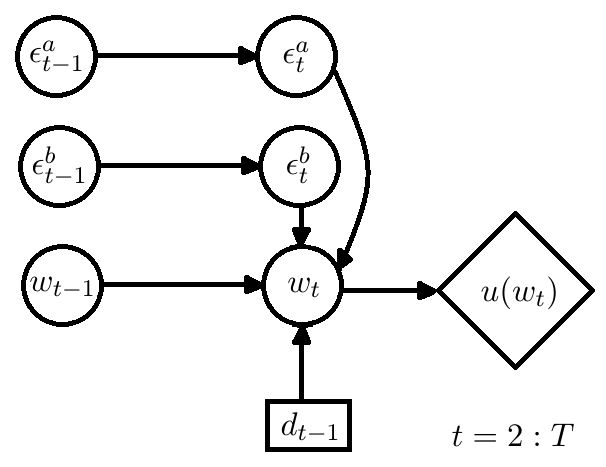
\includegraphics[width=1\textwidth]{c7e13influencediagram}\end{center}
	
\section*{Exercise 7.14}
In order to understand this problem and its utilities and probabilities, we need to look at it from the "player's" perspective. Once he knows that he has a 100 (or $C$ in general) pound cheque, then there are two possibilities (assuming each has equal probability of 0.5). Either the other cheque is 50 ($C/2$) pounds or 200 ($2C$) pounds. Therefore, we have the following expected utilities (where $U(high,change)$ means that the $C$ or 100 pound cheque is the one with twice the amount of the other cheque, which would be 50 pounds):\\
$$U(change) = p(high)U(high,change) + p(low)U(low,change) = 0.5\frac{C}{2} + 0.5*2C = 1.25*C$$
$$U(no\ change) = p(high)U(high,no\ change) + p(low)U(low,no\ change) = 0.5*C + 0.5*C = C$$
Therefore, it is better to change. The same applies if we know the value and it is 100, we simply replace $C = 100$. The confusion regarding this problem is that in reality the "experiment" would be set to either 50-100 or 100-200. In that case (say 50-100), if we had someone change their choice all the time, then it would make no difference. Therefore, if the "player" knew that the case was that it is 50-100, then he would never change if he knew that he got the 100 cheque and if he didn't look at the cheque, then the expected utility would be the same regardless of whether he decides to change or not. The counterintuitive thing about the solution is that, in a sense, it assumes that the experiment can be reproduced many times (as in, every time the player picks a cheque with C or 100 pounds and does not know if the other cheque is C/2 or 2C (50 or 200)), and after running it many times, the player who always changes will have more money than the one who never changes.

\section*{Exercise 9.1}

For the first part of the exercise, we implemented the simple counting algorithm for the maximum likelihood approach. For the second part our MATLAB code prints:\\\\
The probability that there is a fuse assembly malfunction with ML: 1.000000\\\\

For the third part, according to equations 9.4.16 and 9.4.19 and for a flat Beta prior, we simply need to add a 1 to the numerators and a 2 to the denominators during the calculation. Since we have very little data, this in effect reduces the polarization of the probabilities and gives a more conservative probability. MATLAB code prints:\\\\
The probability that there is a fuse assembly malfunction with Bayesian Learning: 0.618615\\\\

For the 4th part after running the code, we manually inspected the final tables and found out that the most likely state is that there is a fuse assembly malfunction and no other problems, just as we programmed MATLAB to print:\\\\
After inspection of the tables of jtpotfullabsorbcond and jtsepfullabsorbcond, the most likely state is that there is a fuse assembly malfunction and no other problems\\\\

For the 5th part, after running the squeezepots and jtree functions from BRML, the junction tree returned is the following (1: Fuse, 2: Drum, 3: Toner, 4: Paper, 5: Roller, 6: Quality, 7: Wrinkled, 8: Multiple Pages):\\

	\begin{center} 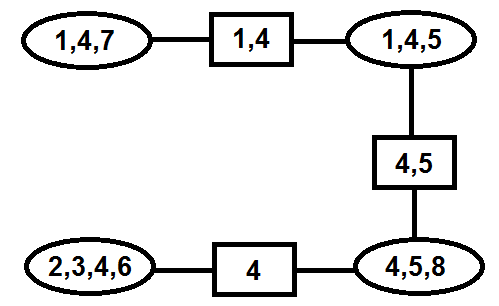
\includegraphics[width=1\textwidth]{c9e1junctiontree}\end{center}
	
Normally we could start the absorption from the 1,4,7 to 1,4,5 and continue. However, we proved in the last assignment, in exercise 6.12, that if a variable exists in only a single clique, then all the potentials that include that variable will exist in that specific clique node. Therefore, whenever we perform the absorption, and we sum over that variable, then it, in effect, gives a new junction tree, which is the marginal of the rest of the variables. Therefore, we can sum over variable 7. This in effect, eliminiates the node 1,4,7 and separator 1,4 and we will then need to "move" the whatever is left (the potentials that we assigned) in node 1,4,7 to node 1,4,5. We can simply think of it as a different assignment of the potentials. We can do the same with the variables 6 and 8. For variable 8, it might not be obvious, since it is in the middle of two clique nodes, but the fact remains that by summing the clique potentials in clique 4,5,8 over variable 8, will result in a junction tree with the marginal of the rest of the variables. In the end, after summing over variables 6,7 and 8 and reassigning the potentials, we are left with the junction tree:\\

	\begin{center} 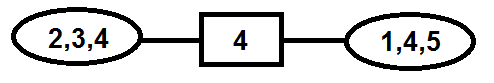
\includegraphics[width=1\textwidth]{c9e1junctiontreefinal}\end{center}
	
	We can now perform the max-absorption algorithm. Once again, after inspecting the final tables, we find out that the most likely state is that there is a fuse malfunction, but also poor paper quality and no other problems:\\

After inspection of the tables of jtpotfullabsorbcond2 and jtsepfullabsorbcond2, the most likely state is that there is a fuse assembly malfunction and poor paper quality and no other problems\\\\

MATLAB code:
\begin{lstlisting}
clear all; clc; close all;
load('printer.mat');
import brml.*

Fuse = 1;
Drum = 2;
Toner = 3;
Paper = 4;
Roller = 5;
Burning = 6;
Quality = 7;
Wrinkled = 8;
MultiplePages = 9;
PaperJam = 10;

fa=1; 
tr=2;

%Part 1
temppot = array(Fuse);
temppot.table(fa) = sum(x(Fuse,:) == fa)/length(x(Fuse,:));
temppot.table(tr) = 1 - temppot.table(fa);
pot{Fuse} = temppot;

temppot = array(Drum);
temppot.table(fa) = sum(x(Drum,:) == fa)/length(x(Drum,:));
temppot.table(tr) = 1 - temppot.table(fa);
pot{Drum} = temppot;

temppot = array(Toner);
temppot.table(fa) = sum(x(Toner,:) == fa)/length(x(Toner,:));
temppot.table(tr) = 1 - temppot.table(fa);
pot{Toner} = temppot;

temppot = array(Paper);
temppot.table(fa) = sum(x(Paper,:) == fa)/length(x(Paper,:));
temppot.table(tr) = 1 - temppot.table(fa);
pot{Paper} = temppot;

temppot = array(Roller);
temppot.table(fa) = sum(x(Roller,:) == fa)/length(x(Roller,:));
temppot.table(tr) = 1 - temppot.table(fa);
pot{Roller} = temppot;

temppot = array([Burning Fuse]);
temppot.table(fa,fa) = sum(x(Burning,x(Fuse,:) == fa)==fa)/length(find(x(Fuse,:) == fa));
temppot.table(fa,tr) = sum(x(Burning,x(Fuse,:) == tr)==fa)/length(find(x(Fuse,:) == tr));
temppot.table(tr,:) = 1 - temppot.table(fa,:);
pot{Burning} = condpot(temppot,Burning,Fuse);

temppot = array([Quality Drum Toner Paper]);
temppot.table(fa,fa,fa,fa) = sum(x(Quality,x(Drum,:) == fa & x(Toner,:) == fa & x(Paper,:) == fa)==fa)/length(find((x(Drum,:) == fa & x(Toner,:) == fa & x(Paper,:) == fa)==fa));
temppot.table(fa,fa,fa,tr) = sum(x(Quality,x(Drum,:) == fa & x(Toner,:) == fa & x(Paper,:) == tr)==fa)/length(find((x(Drum,:) == fa & x(Toner,:) == fa & x(Paper,:) == tr)==fa));
temppot.table(fa,fa,tr,fa) = sum(x(Quality,x(Drum,:) == fa & x(Toner,:) == tr & x(Paper,:) == fa)==fa)/length(find((x(Drum,:) == fa & x(Toner,:) == tr & x(Paper,:) == fa)==fa));
temppot.table(fa,fa,tr,tr) = sum(x(Quality,x(Drum,:) == fa & x(Toner,:) == tr & x(Paper,:) == tr)==fa)/length(find((x(Drum,:) == fa & x(Toner,:) == tr & x(Paper,:) == tr)==fa));
temppot.table(fa,tr,fa,fa) = sum(x(Quality,x(Drum,:) == tr & x(Toner,:) == fa & x(Paper,:) == fa)==fa)/length(find((x(Drum,:) == tr & x(Toner,:) == fa & x(Paper,:) == fa)==fa));
temppot.table(fa,tr,fa,tr) = sum(x(Quality,x(Drum,:) == tr & x(Toner,:) == fa & x(Paper,:) == tr)==fa)/length(find((x(Drum,:) == tr & x(Toner,:) == fa & x(Paper,:) == tr)==fa));
temppot.table(fa,tr,tr,fa) = sum(x(Quality,x(Drum,:) == tr & x(Toner,:) == tr & x(Paper,:) == fa)==fa)/length(find((x(Drum,:) == tr & x(Toner,:) == tr & x(Paper,:) == fa)==fa));
temppot.table(fa,tr,tr,tr) = sum(x(Quality,x(Drum,:) == tr & x(Toner,:) == tr & x(Paper,:) == tr)==fa)/length(find((x(Drum,:) == tr & x(Toner,:) == tr & x(Paper,:) == tr)==fa));
temppot.table(tr,:,:,:) = 1 - temppot.table(fa,:,:,:);
pot{Quality} = condpot(temppot,Quality,[Drum Toner Paper]);

temppot = array([Wrinkled Fuse Paper]);
temppot.table(fa,fa,fa) = sum(x(Wrinkled,x(Fuse,:) == fa & x(Paper,:) == fa)==fa)/length(find((x(Fuse,:) == fa & x(Paper,:) == fa)==fa));
temppot.table(fa,fa,tr) = sum(x(Wrinkled,x(Fuse,:) == fa & x(Paper,:) == tr)==fa)/length(find((x(Fuse,:) == fa & x(Paper,:) == tr)==fa));
temppot.table(fa,tr,fa) = sum(x(Wrinkled,x(Fuse,:) == tr & x(Paper,:) == fa)==fa)/length(find((x(Fuse,:) == tr & x(Paper,:) == fa)==fa));
temppot.table(fa,tr,tr) = sum(x(Wrinkled,x(Fuse,:) == tr & x(Paper,:) == tr)==fa)/length(find((x(Fuse,:) == tr & x(Paper,:) == tr)==fa));
temppot.table(tr,:,:) = 1 - temppot.table(fa,:,:);
pot{Wrinkled} = condpot(temppot,Wrinkled,[Fuse Paper]);

temppot = array([MultiplePages Paper Roller]);
temppot.table(fa,fa,fa) = sum(x(MultiplePages,x(Paper,:) == fa & x(Roller,:) == fa)==fa)/length(find((x(Paper,:) == fa & x(Roller,:) == fa)==fa));
temppot.table(fa,fa,tr) = sum(x(MultiplePages,x(Paper,:) == fa & x(Roller,:) == tr)==fa)/length(find((x(Paper,:) == fa & x(Roller,:) == tr)==fa));
temppot.table(fa,tr,fa) = sum(x(MultiplePages,x(Paper,:) == tr & x(Roller,:) == fa)==fa)/length(find((x(Paper,:) == tr & x(Roller,:) == fa)==fa));
temppot.table(fa,tr,tr) = sum(x(MultiplePages,x(Paper,:) == tr & x(Roller,:) == tr)==fa)/length(find((x(Paper,:) == tr & x(Roller,:) == tr)==fa));
temppot.table(tr,:,:) = 1 - temppot.table(fa,:,:);
pot{MultiplePages} = condpot(temppot,MultiplePages,[Paper Roller]);

temppot = array([PaperJam Fuse Roller]);
temppot.table(fa,fa,fa) = sum(x(PaperJam,x(Fuse,:) == fa & x(Roller,:) == fa)==fa)/length(find((x(Fuse,:) == fa & x(Roller,:) == fa)==fa));
temppot.table(fa,fa,tr) = sum(x(PaperJam,x(Fuse,:) == fa & x(Roller,:) == tr)==fa)/length(find((x(Fuse,:) == fa & x(Roller,:) == tr)==fa));
temppot.table(fa,tr,fa) = sum(x(PaperJam,x(Fuse,:) == tr & x(Roller,:) == fa)==fa)/length(find((x(Fuse,:) == tr & x(Roller,:) == fa)==fa));
temppot.table(fa,tr,tr) = sum(x(PaperJam,x(Fuse,:) == tr & x(Roller,:) == tr)==fa)/length(find((x(Fuse,:) == tr & x(Roller,:) == tr)==fa));
temppot.table(tr,:,:) = 1 - temppot.table(fa,:,:);
pot{PaperJam} = condpot(temppot,PaperJam,[Fuse Roller]);

%Part 2
Jointpot = multpots(pot);
FuseML = setpot(sumpot(Jointpot,[Drum Toner Paper Roller]),[Burning PaperJam Quality Wrinkled MultiplePages],[tr tr fa fa fa]);
FuseML.table = FuseML.table/sum(FuseML.table);
fprintf('The probability that there is a fuse assembly malfunction with ML: %f\n',FuseML.table(tr));

%Part 3
temppot = array(Fuse);
temppot.table(fa) = (1+sum(x(Fuse,:) == fa))/(2+length(x(Fuse,:)));
temppot.table(tr) = 1 - temppot.table(fa);
Bayespot{Fuse} = temppot;

temppot = array(Drum);
temppot.table(fa) = (1+sum(x(Drum,:) == fa))/(2+length(x(Drum,:)));
temppot.table(tr) = 1 - temppot.table(fa);
Bayespot{Drum} = temppot;

temppot = array(Toner);
temppot.table(fa) = (1+sum(x(Toner,:) == fa))/(2+length(x(Toner,:)));
temppot.table(tr) = 1 - temppot.table(fa);
Bayespot{Toner} = temppot;

temppot = array(Paper);
temppot.table(fa) = (1+sum(x(Paper,:) == fa))/(2+length(x(Paper,:)));
temppot.table(tr) = 1 - temppot.table(fa);
Bayespot{Paper} = temppot;

temppot = array(Roller);
temppot.table(fa) = (1+sum(x(Roller,:) == fa))/(2+length(x(Roller,:)));
temppot.table(tr) = 1 - temppot.table(fa);
Bayespot{Roller} = temppot;

temppot = array([Burning Fuse]);
temppot.table(fa,fa) = (1+sum(x(Burning,x(Fuse,:) == fa)==fa))/(2+length(find(x(Fuse,:) == fa)));
temppot.table(fa,tr) = (1+sum(x(Burning,x(Fuse,:) == tr)==fa))/(2+length(find(x(Fuse,:) == tr)));
temppot.table(tr,:) = 1 - temppot.table(fa,:);
Bayespot{Burning} = condpot(temppot,Burning,Fuse);

temppot = array([Quality Drum Toner Paper]);
temppot.table(fa,fa,fa,fa) = (1+sum(x(Quality,x(Drum,:) == fa & x(Toner,:) == fa & x(Paper,:) == fa)==fa))/(2+length(find((x(Drum,:) == fa & x(Toner,:) == fa & x(Paper,:) == fa)==fa)));
temppot.table(fa,fa,fa,tr) = (1+sum(x(Quality,x(Drum,:) == fa & x(Toner,:) == fa & x(Paper,:) == tr)==fa))/(2+length(find((x(Drum,:) == fa & x(Toner,:) == fa & x(Paper,:) == tr)==fa)));
temppot.table(fa,fa,tr,fa) = (1+sum(x(Quality,x(Drum,:) == fa & x(Toner,:) == tr & x(Paper,:) == fa)==fa))/(2+length(find((x(Drum,:) == fa & x(Toner,:) == tr & x(Paper,:) == fa)==fa)));
temppot.table(fa,fa,tr,tr) = (1+sum(x(Quality,x(Drum,:) == fa & x(Toner,:) == tr & x(Paper,:) == tr)==fa))/(2+length(find((x(Drum,:) == fa & x(Toner,:) == tr & x(Paper,:) == tr)==fa)));
temppot.table(fa,tr,fa,fa) = (1+sum(x(Quality,x(Drum,:) == tr & x(Toner,:) == fa & x(Paper,:) == fa)==fa))/(2+length(find((x(Drum,:) == tr & x(Toner,:) == fa & x(Paper,:) == fa)==fa)));
temppot.table(fa,tr,fa,tr) = (1+sum(x(Quality,x(Drum,:) == tr & x(Toner,:) == fa & x(Paper,:) == tr)==fa))/(2+length(find((x(Drum,:) == tr & x(Toner,:) == fa & x(Paper,:) == tr)==fa)));
temppot.table(fa,tr,tr,fa) = (1+sum(x(Quality,x(Drum,:) == tr & x(Toner,:) == tr & x(Paper,:) == fa)==fa))/(2+length(find((x(Drum,:) == tr & x(Toner,:) == tr & x(Paper,:) == fa)==fa)));
temppot.table(fa,tr,tr,tr) = (1+sum(x(Quality,x(Drum,:) == tr & x(Toner,:) == tr & x(Paper,:) == tr)==fa))/(2+length(find((x(Drum,:) == tr & x(Toner,:) == tr & x(Paper,:) == tr)==fa)));
temppot.table(tr,:,:,:) = 1 - temppot.table(fa,:,:,:);
Bayespot{Quality} = condpot(temppot,Quality,[Drum Toner Paper]);

temppot = array([Wrinkled Fuse Paper]);
temppot.table(fa,fa,fa) = (1+sum(x(Wrinkled,x(Fuse,:) == fa & x(Paper,:) == fa)==fa))/(2+length(find((x(Fuse,:) == fa & x(Paper,:) == fa)==fa)));
temppot.table(fa,fa,tr) = (1+sum(x(Wrinkled,x(Fuse,:) == fa & x(Paper,:) == tr)==fa))/(2+length(find((x(Fuse,:) == fa & x(Paper,:) == tr)==fa)));
temppot.table(fa,tr,fa) = (1+sum(x(Wrinkled,x(Fuse,:) == tr & x(Paper,:) == fa)==fa))/(2+length(find((x(Fuse,:) == tr & x(Paper,:) == fa)==fa)));
temppot.table(fa,tr,tr) = (1+sum(x(Wrinkled,x(Fuse,:) == tr & x(Paper,:) == tr)==fa))/(2+length(find((x(Fuse,:) == tr & x(Paper,:) == tr)==fa)));
temppot.table(tr,:,:) = 1 - temppot.table(fa,:,:);
Bayespot{Wrinkled} = condpot(temppot,Wrinkled,[Fuse Paper]);

temppot = array([MultiplePages Paper Roller]);
temppot.table(fa,fa,fa) = (1+sum(x(MultiplePages,x(Paper,:) == fa & x(Roller,:) == fa)==fa))/(2+length(find((x(Paper,:) == fa & x(Roller,:) == fa)==fa)));
temppot.table(fa,fa,tr) = (1+sum(x(MultiplePages,x(Paper,:) == fa & x(Roller,:) == tr)==fa))/(2+length(find((x(Paper,:) == fa & x(Roller,:) == tr)==fa)));
temppot.table(fa,tr,fa) = (1+sum(x(MultiplePages,x(Paper,:) == tr & x(Roller,:) == fa)==fa))/(2+length(find((x(Paper,:) == tr & x(Roller,:) == fa)==fa)));
temppot.table(fa,tr,tr) = (1+sum(x(MultiplePages,x(Paper,:) == tr & x(Roller,:) == tr)==fa))/(2+length(find((x(Paper,:) == tr & x(Roller,:) == tr)==fa)));
temppot.table(tr,:,:) = 1 - temppot.table(fa,:,:);
Bayespot{MultiplePages} = condpot(temppot,MultiplePages,[Paper Roller]);

temppot = array([PaperJam Fuse Roller]);
temppot.table(fa,fa,fa) = (1+sum(x(PaperJam,x(Fuse,:) == fa & x(Roller,:) == fa)==fa))/(2+length(find((x(Fuse,:) == fa & x(Roller,:) == fa)==fa)));
temppot.table(fa,fa,tr) = (1+sum(x(PaperJam,x(Fuse,:) == fa & x(Roller,:) == tr)==fa))/(2+length(find((x(Fuse,:) == fa & x(Roller,:) == tr)==fa)));
temppot.table(fa,tr,fa) = (1+sum(x(PaperJam,x(Fuse,:) == tr & x(Roller,:) == fa)==fa))/(2+length(find((x(Fuse,:) == tr & x(Roller,:) == fa)==fa)));
temppot.table(fa,tr,tr) = (1+sum(x(PaperJam,x(Fuse,:) == tr & x(Roller,:) == tr)==fa))/(2+length(find((x(Fuse,:) == tr & x(Roller,:) == tr)==fa)));
temppot.table(tr,:,:) = 1 - temppot.table(fa,:,:);
Bayespot{PaperJam} = condpot(temppot,PaperJam,[Fuse Roller]);

BayesJointpot = multpots(Bayespot);
FuseBayes = setpot(sumpot(BayesJointpot,[Drum Toner Paper Roller]),[Burning PaperJam Quality Wrinkled MultiplePages],[tr tr fa fa fa]);
FuseBayes.table = FuseBayes.table/sum(FuseBayes.table);
fprintf('The probability that there is a fuse assembly malfunction with Bayesian Learning: %f\n',FuseBayes.table(tr));

%part 4
for i = 1:1:10
    potcond{i} = setpot(Bayespot{i},[Burning PaperJam Quality Wrinkled MultiplePages], [tr tr fa fa fa]);
end
[newpot, ~, ~, ~] = squeezepots(potcond);
[jtpotcond, jtsepcond, infostructcond]=jtree(newpot);
[jtpotfullabsorbcond, jtsepfullabsorbcond, Zcond]=absorption(jtpotcond,jtsepcond,infostructcond,'max');
fprintf('After inspection of the tables of jtpotfullabsorbcond and jtsepfullabsorbcond, the most likely state is that there is a fuse assembly malfunction and no other problems\n');

%part 5
for i = 1:1:10
    potcond2{i} = setpot(Bayespot{i},[Burning PaperJam], [tr tr]);
end
[newpot2, ~, ~, ~] = squeezepots(potcond2);
[jtpotcond2, jtsepcond2, infostructcond2]=jtree(newpot2);
for i = 1:1:length(jtpotcond2)
    jtpotcond2{i} = sumpot(jtpotcond2{i},[6 7 8]);
end
jtpotcond2{1} = multpots([jtpotcond2{1} jtpotcond2{2} jtpotcond2{3}]);
jtpotcond2{2} = jtpotcond2{4};
jtpotcond2 = jtpotcond2([1 2]);
jtsepcond2 = jtsepcond2(1);
infostructcond2.cliquevariables{1} = [1 4 5];
infostructcond2.cliquevariables{2} = [2 3 4];
infostructcond2.cliquevariables = infostructcond2.cliquevariables([1 2]);
infostructcond2.separator = infostructcond2.separator([3]);
infostructcond2.cliquetree = sparse([0 1;1 0]);
infostructcond2.sepind = sparse([1 2], [2 1], [1 1]);
infostructcond2.EliminationSchedule = [1 2];
[jtpotfullabsorbcond2, jtsepfullabsorbcond2, Zcond2]=absorption(jtpotcond2,jtsepcond2,infostructcond2,'max');
fprintf('After inspection of the tables of jtpotfullabsorbcond2 and jtsepfullabsorbcond2, the most likely state is that there is a fuse assembly malfunction and poor paper quality and no other problems\n');
\end{lstlisting}

\section*{Exercise 9.9}

Starting with equation 9.4.53, we can use the equation 8.3.30 for each of the normalization constants of the Dirichlet distributions:

\begin{align*}
p(D)&=\prod_k\prod_j\frac{Z(\mathbf{u'}(v_k;j))}{Z(\mathbf{u}(v_k;j))}\\
Z(\mathbf{u})&=\frac{\prod_i\Gamma(u_i)}{\Gamma(\sum_iu_i)}\\
&\text{Therefore:}\\
Z(\mathbf{u'}(v_k;j))&=\frac{\prod_i\Gamma(u_i'(v_k;j))}{\Gamma(\sum_iu_i'(v_k;j))}\\
Z(\mathbf{u}(v_k;j))&=\frac{\prod_i\Gamma(u_i(v_k;j))}{\Gamma(\sum_iu_i(v_k;j))}\\
&\text{So, by inputting them into the initial equation we get:}\\
p(D)&=\prod_k\prod_j\frac{\prod_i\Gamma(u_i'(v_k;j))}{\Gamma(\sum_iu_i'(v_k;j))}\frac{\Gamma(\sum_iu_i(v_k;j))}{\prod_i\Gamma(u_i(v_k;j))}=\\
p(D)&=\prod_k\prod_j\frac{\Gamma(\sum_iu_i(v_k;j))}{\Gamma(\sum_iu_i'(v_k;j))}\frac{\prod_i\Gamma(u_i'(v_k;j))}{\prod_i\Gamma(u_i(v_k;j))}=\\
p(D)&=\prod_k\prod_j\frac{\Gamma(\sum_iu_i(v_k;j))}{\Gamma(\sum_iu_i'(v_k;j))}\prod_i\left[\frac{\Gamma(u_i'(v_k;j))}{\Gamma(u_i(v_k;j))}\right]
\end{align*}

\section*{Exercise 9.10}

Part 1\\
Given the arbitrary ancestral ordering a: $x_1,x_2,x_3,x_4,x_5,x_6,x_7,x_8$, the number of belief networks will be: $\#N_a=\#a(x_1)*\#a(x_2)*...*\#a(x_8)$, where $\#a(x_i)$ is the number of different combinations/possible ancestors of $x_i$. As such, we have:
\begin{align*}
\#a(x_1)&=1=1\\
\#a(x_2)&=1+1=2\\
\#a(x_3)&=1+\binom 21 +\binom 22=4\\
\#a(x_4)&=1+\binom 31 +\binom 32=7\\
\#a(x_5)&=1+\binom 41 +\binom 42=11\\
\#a(x_6)&=1+\binom 51 +\binom 52=16\\
\#a(x_7)&=1+\binom 61 +\binom 62=22\\
\#a(x_8)&=1+\binom 71 +\binom 72=29\\
&\text{Therefore:}\\
\#N_a&=1*2*4*7*11*16*22*29=6288128
\end{align*}

Part 2\\
Due to the decomposability of the BD score, we can optimize it for each variable independently. Therefore the total number of belief networks we will need to examine is:
$$O(N_a)=\#a(x_1) + (\#a(x_2)-1)+...+(\#a(x_8)-1)= 1+1+3+6+10+15+21+29=86 seconds$$
The fact that we only need to sum instead of multiply is thanks to the decomposability property. The minus 1 to each element can be understood if, for example, we only have 3 variables. In this case we could give a state for what parents each variable has. For example state 111 means that none of the variables have a parent, whereas state 121 means that the second variable has the first variable as a parent. We would thus first examine state 111. Then state 121. By now, we would know the parents of the first and second variable. Let us assume that the second variable also has no parents. We would then proceed to check states 112, 113 and 114. Due to the fact that we don't need to recheck state 111 is the reason for the minus one.\\

Part 3\\
The only thing left is to find all the permutations of ancestral orderings. Therefore the total time will be $O(N) = 8!O(N_a)=3467520 seconds$

\section*{Exercise 9.13}

MATLAB code:
\begin{lstlisting}
function A = ChowLiu(X)
import brml.*
[D,N] = size(X);
W = zeros(D);
%Find all mutual information
for i = 1:1:D
    for j = 1:1:D
        W(i,j) = MIemp(X(i,:),X(j,:),max(X(i,:)),max(X(j,:)));
    end
end
%Spanning tree
[Atree, ~, ~]=spantree(W);
%DAG
A = Atree;
Ordering = 1;
for counter = 1:1:D
    node = Ordering(counter);
    A(setdiff(1:D,Ordering(1:counter)),node) = 0;
    Ordering = [Ordering find(A(node,:))];
end
drawNet(A);
end
\end{lstlisting}

The code to convert the tree to a DAG finds the ancestral ordering of the variables and on every iteration, makes sure that no "younger" nodes point to the current "older" node.

The Chow Liu tree we get is:

	\begin{center} 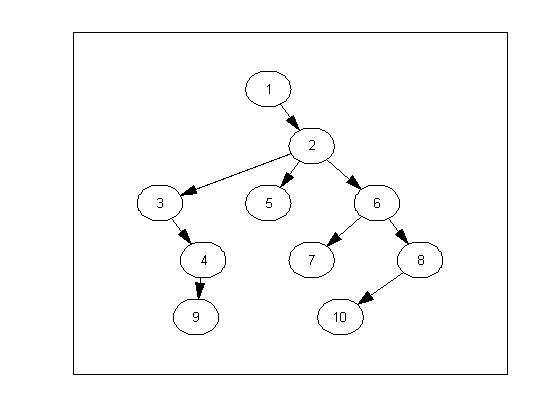
\includegraphics[width=1\textwidth]{c9e13chowliutree}\end{center}

\section*{Exercise 10.3}
MATLAB code:
\begin{lstlisting}
clear all; clc; close all;
import brml.*
xP = [1 0 1 1 1 0 1 1;
      0 0 0 1 0 0 1 1;
      1 0 0 1 1 0 1 0;
      0 1 0 0 1 1 0 1;
      0 0 0 1 1 0 1 1;
      0 0 0 1 1 0 0 1]';
xS = [1 1 0 0 0 0 0 0;
      0 0 1 0 0 0 0 0;
      1 1 0 1 0 0 0 0;
      1 1 0 1 0 0 0 1;
      1 1 0 1 1 0 0 0;
      0 0 0 1 0 1 0 0;
      1 1 1 1 1 0 1 0]';
[pP, pS, mP, mS]=NaiveBayesTrain(xP,xS);
x = [1 0 0 1 1 1 1 0]';
px=NaiveBayesTest(x,pP,pS,mP,mS);
fprintf('The probability that x=(1,0,0,1,1,1,1,0) is about politics is: %f.\n',px(1));
\end{lstlisting}

The probability that x=(1,0,0,1,1,1,1,0) is about politics is: 0.830599.

\section*{Exercise 10.5}

Part 1\\
According to equations (10.2.5) and (10.2.7) we have:
\begin{align*}
p(c=1) &=  \frac{\sum_{n=1}^N \mathbbm{I}{[c^n=1]}}{N}\\
p(x_i=1|c=1) &=  \frac{\sum_{n=1}^N \mathbbm{I}{[x_i^n=1,c^n=1]}}{\sum_{n=1}^N \mathbbm{I}{[x_i^n=1,c^n=1]}+\mathbbm{I}{[x_i^n=0,c^n=1]}},i=1,...,D\\
p(x_i=1|c=0) &=  \frac{\sum_{n=1}^N \mathbbm{I}{[x_i^n=1,c^n=0]}}{\sum_{n=1}^N \mathbbm{I}{[x_i^n=1,c^n=0]}+\mathbbm{I}{[x_i^n=0,c^n=0]}},i=1,...,D
\end{align*}

Part 2\\
As described in the Classification boundary section of the book, given an input $x^\ast$, we can classify it to be in class $c=1$ if (equation 10.2.10):
\begin{align*}
p(c=1|x^\ast)&>p(c=0|x^\ast)\\
\sum_{i=1}^D\log p(x_i^\ast|c=1)+\log p(c=1)&>\sum_{i=1}^D\log p(x_i^\ast|c=0)+\log p(c=0)
\end{align*}

Otherwise, we classify it as belonging to class $c=0$.\\

Part 3\\
If we assume that $x_4=1$ means that the word 'viagra' is present in the e-mail, then if it never appears in the training data, it means that:
$$p(x_4=1|c=1) =  \frac{\sum_{n=1}^N \mathbbm{I}{[x_4^n=1,c^n=1]}}{\sum_{n=1}^N \mathbbm{I}{[x_4^n=1,c^n=1]}+\mathbbm{I}{[x_4^n=0,c^n=1]}}=\frac{0}{0+N}=0$$
Which means that:
\begin{align*}
p(c=1|x^\ast)&=\frac{p(x^\ast|c=1)p(c=1)}{p(x^\ast)}=\prod_{i=1}^Dp(x_i=x_i^\ast|c=1)\frac{p(c=1)}{p(x^\ast)}=0
\end{align*}
The above is equal to 0 since $x_4^\ast=1$ and $p(x_4=x_4^\ast|c=1)=p(x_4=1|c=1)=0$. This means that an e-mail containing the word 'viagra' will never be classified as spam with the current training performed. By using a Bayesian approach, as is explained in chapter 10.3, we can use Beta distribution priors and change the learning of the tables to, for example with a flat prior, add a 1 to the numerator and a 2 to the denominator, just as in exercise 9.1 part 3. This, essentially has the effect of enforcing the training to happen as if in the training data all words appear and also are absent at least once. One could produce the same result by adding the e-mails of all ones and all zeros: [1,1,...,1] and [0,0,...,0] to both spam and not-spam training data sets.\\
Therefore, a spammer should in general use words which do not appear, or rarely appear, in typical spam e-mails. They could also slightly change the words, e.g. 'v1agra' instead of 'viagra'. Also, depending on how "online" the training is(as in, it keeps retraining itself with the new data), one could possibly send a lot of spam with words he does not intend to use in his real spam e-mail and lacking the words that he intends to use in his real spam e-mail, which would polarize the classifier more towards not classifying his real spam e-mails as such.

\end{document}





















